\subsubsection{\emph{Development View}}
\label{subsubsec:development-view}
\emph{Development view} mendefinisikan organisasi sistem dari sudut pandang pengembang. \emph{Development view} membuat pengembang dapat memahami struktur sistem hingga level komponen dan bagaimana komponen tersebut berinteraksi satu sama lain. \autoref{fig:component-diagram} menunjukkan \emph{component diagram} sistem pencatatan pengeluaran berbasis \emph{mobile}. Diagram ini menunjukkan bagaimana sistem dibagi menjadi beberapa komponen, yaitu aplikasi \emph{mobile}, layanan \emph{backend}, model internal, dan model \emph{deployed}. Setiap komponen memiliki tanggung jawab dan interaksi yang jelas dengan kompoenen lainnya untuk memungkinkan pengembangan sistem yang lebih terstruktur.

\begin{figure}[htbp]
    \centering
    % 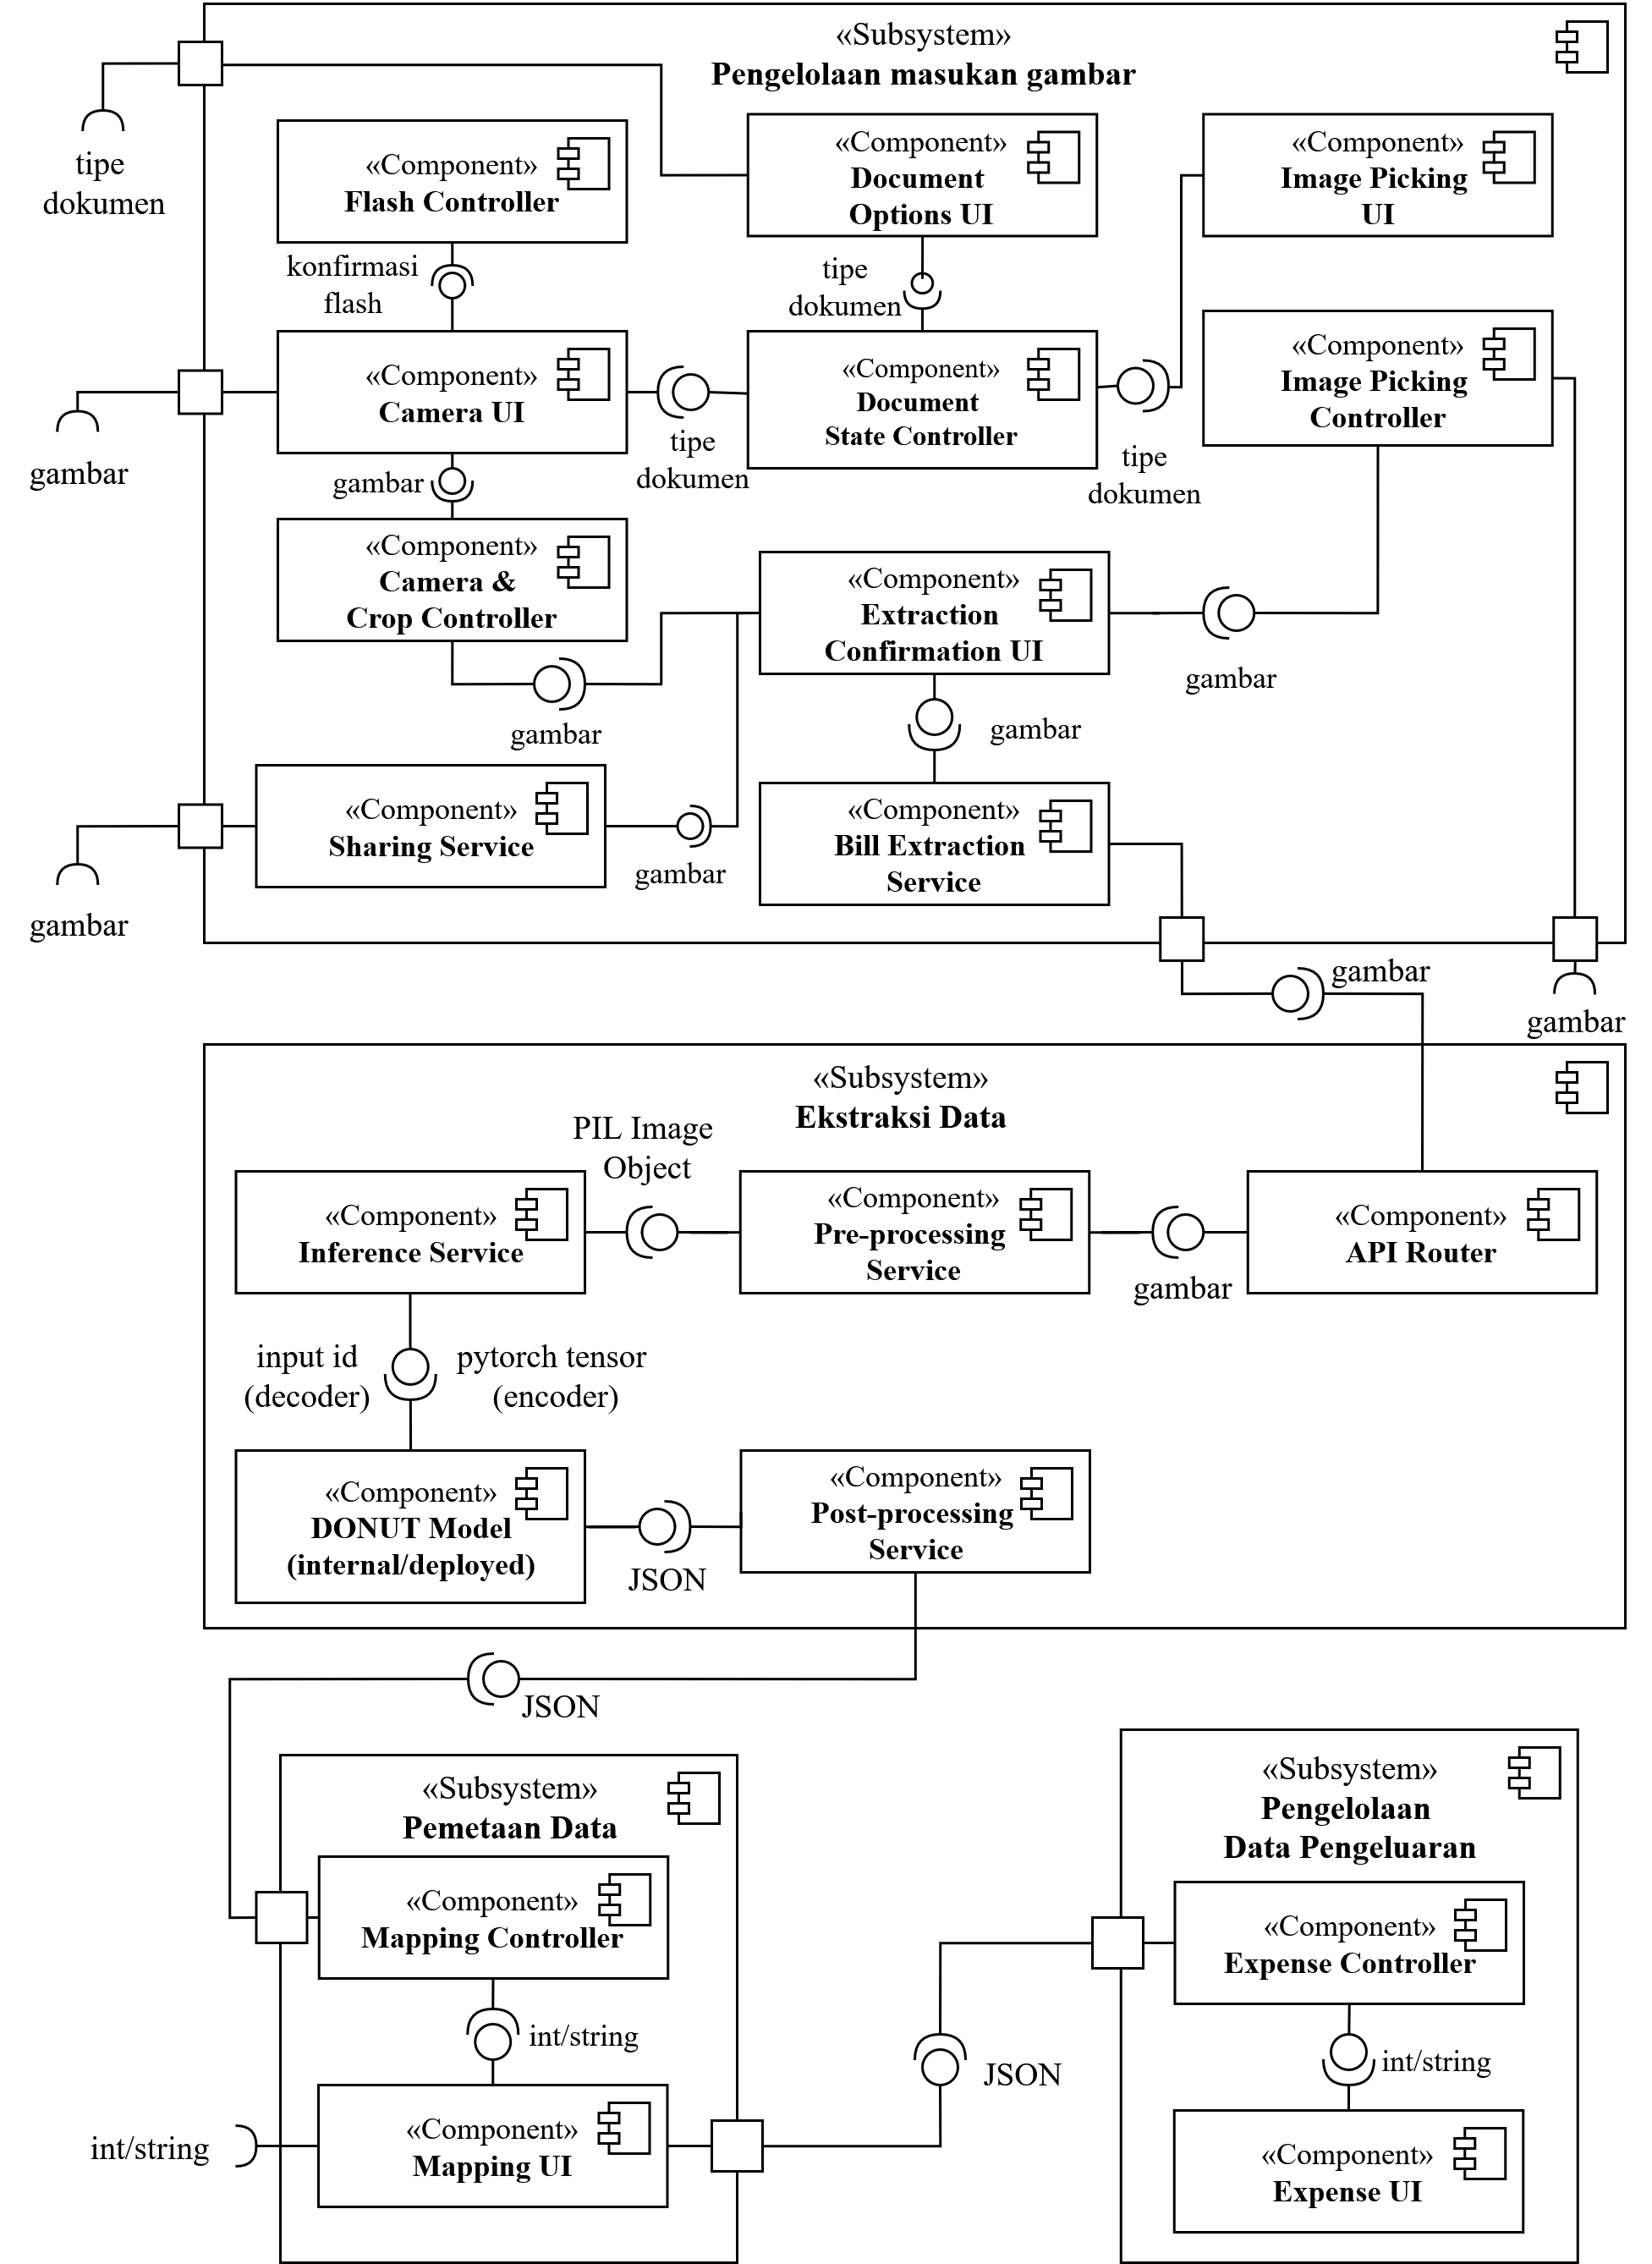
\includegraphics[width=1\textwidth]{images/component-diagram.png}
    \caption{\emph{Component diagram} sistem pencatatan pengeluaran berbasis \emph{mobile}}
    \label{fig:component-diagram}
\end{figure}